\FloatBarrier

\begin{figure}[h!]
	\centering
	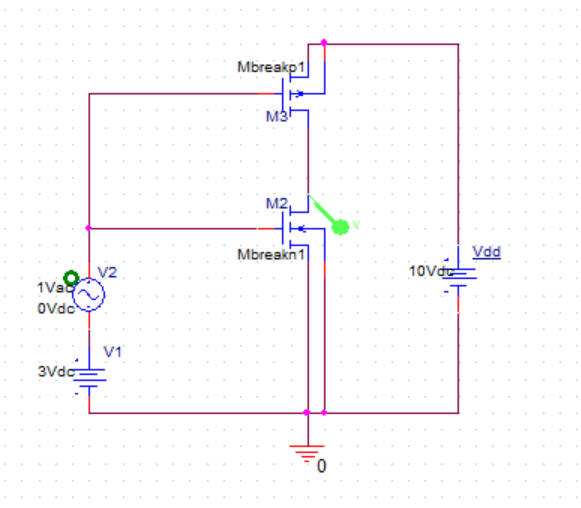
\includegraphics[scale=0.75]{./images/circuit4.PNG}
	\caption{Common-Source Amplifier with Active Load}
	\label{fig:circuit4}
\end{figure}

\FloatBarrier

\FloatBarrier

\begin{figure}[h!]
	\centering
	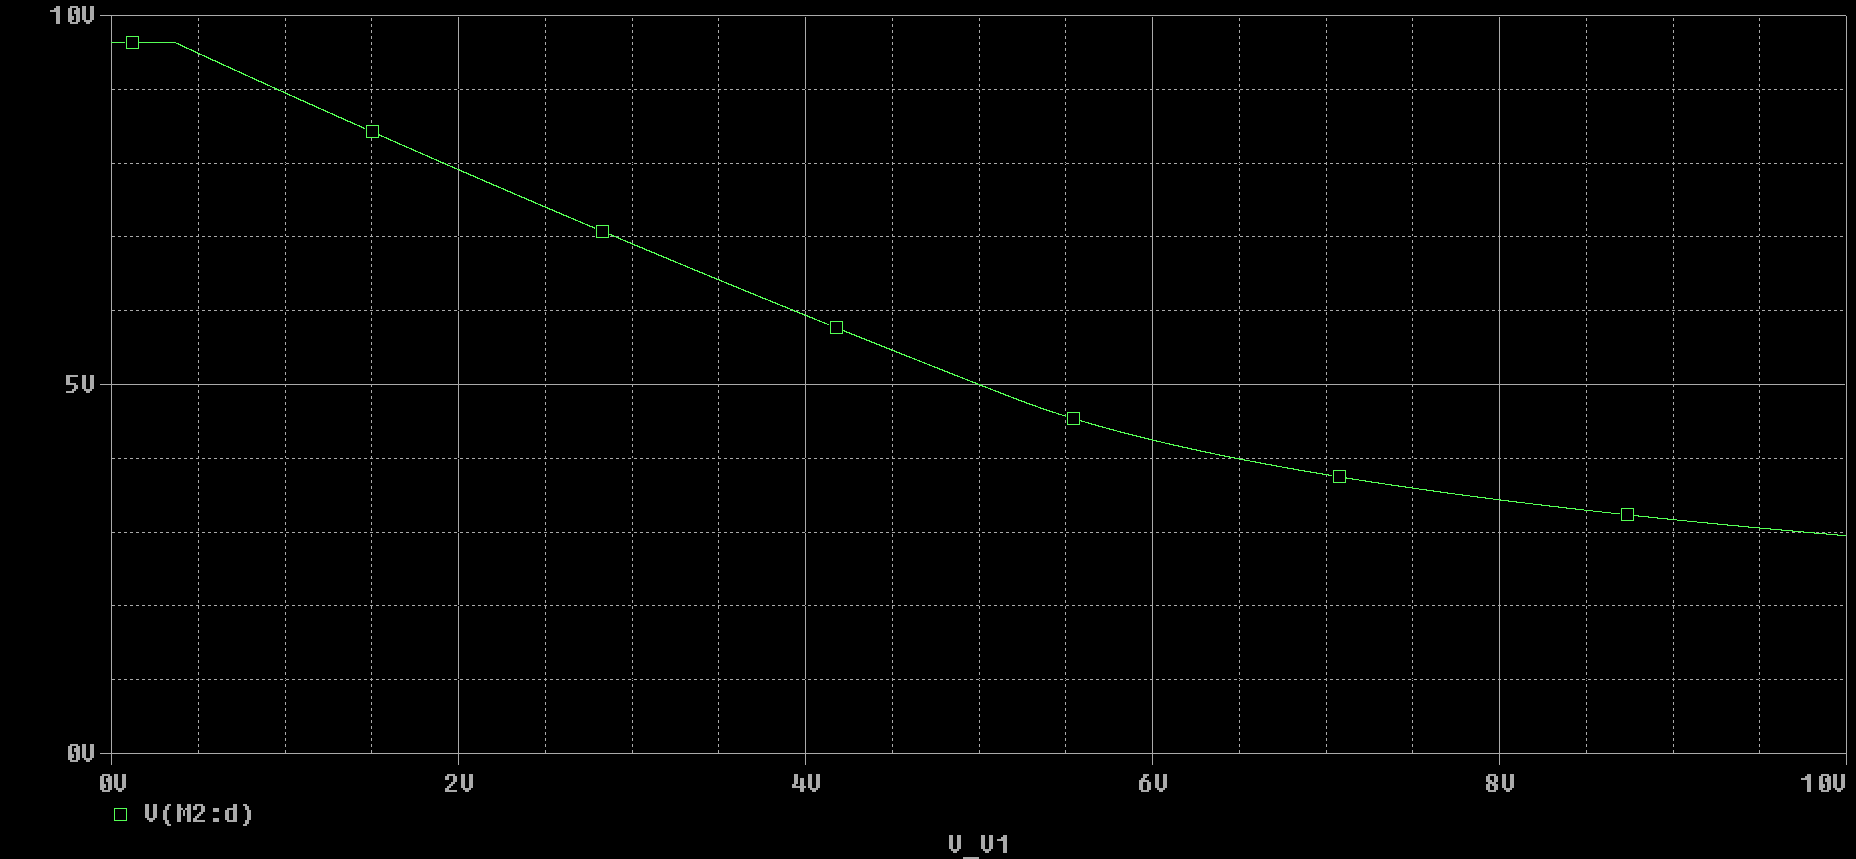
\includegraphics[scale=0.50]{./images/dc_sweep.PNG}
	\caption{Voltage Transfer Characteristic}
	\label{fig:dc_sweep}
\end{figure}

\FloatBarrier

% How does V_out change with biasing?
When the bias voltage $V_{GS}$ is increased, $V_{out}$'s bias is decreased. For sufficiently low $V_{GS}$ values, the output is biased at $5$\si{\volt}. For sufficiently high $V_{GS}$ values, the output is biased near $3$\si{\volt}.

% Compare to your result in part 1
% Which is a better choice? NMOS acting as a resistor or a true resistor?
After the bottom transistor exits cutoff, the common-source amplifiers with both passive and active loads exhibit linear behavior until a certain point. However, now that an NMOS is being used in place of a resistor, the slope is much lower in magnitude. Input AC signals must be varied more in order to achieve the same output voltage. As a result, the amplifier is subject to more distortion. Moreover, this amplifier would be a very poor inverter due to its gradual decline from a "1" to a "0". \uline{Therefore, if the option is available, a true resistor is preferred to an NMOS acting as a resistor.}
